\documentclass[11pt]{article}

% Change "review" to "final" to generate the final (sometimes called camera-ready) version.
% Change to "preprint" to generate a non-anonymous version with page numbers.
% \usepackage[review]{acl}
\usepackage[preprint]{acl}

% Standard package includes
\usepackage{times}
\usepackage{latexsym}

% For proper rendering and hyphenation of words containing Latin characters (including in bib files)
\usepackage[T1]{fontenc}
% For Vietnamese characters
% \usepackage[T5]{fontenc}
% See https://www.latex-project.org/help/documentation/encguide.pdf for other character sets

% This assumes your files are encoded as UTF8
\usepackage[utf8]{inputenc}

% This is not strictly necessary, and may be commented out,
% but it will improve the layout of the manuscript,
% and will typically save some space.
\usepackage{microtype}

% This is also not strictly necessary, and may be commented out.
% However, it will improve the aesthetics of text in
% the typewriter font.
\usepackage{inconsolata}

%Including images in your LaTeX document requires adding
%additional package(s)
\usepackage{graphicx}
\usepackage{float}

% If the title and author information does not fit in the area allocated, uncomment the following
%
%\setlength\titlebox{<dim>}
%
% and set <dim> to something 5cm or larger.

\title{Handwritten Mathematical Expression Recognition Using Convolutional Neural Networks}

% Author information can be set in various styles:
% For several authors from the same institution:
% \author{Author 1 \and ... \and Author n \\
%         Address line \\ ... \\ Address line}
% if the names do not fit well on one line use
%         Author 1 \\ {\bf Author 2} \\ ... \\ {\bf Author n} \\
% For authors from different institutions:
% \author{Author 1 \\ Address line \\  ... \\ Address line
%         \And  ... \And
%         Author n \\ Address line \\ ... \\ Address line}
% To start a separate ``row'' of authors use \AND, as in
% \author{Author 1 \\ Address line \\  ... \\ Address line
%         \AND
%         Author 2 \\ Address line \\ ... \\ Address line \And
%         Author 3 \\ Address line \\ ... \\ Address line}

% Bios of the researchers! Include your name, NetID, department, and year in the
% program. Also list what each team member will likely be responsible for or how you
% plan to divide the work fairly.

\author{
    Nathan Emeott \\
    Computer Science \\
    Junior \\
    \\\And
    Patrick Schrems \\
    Computational \& \\Applied Mathematics \\
    and Computer Science \\
    Junior \\
    \\\And
    Mihir Patel \\
    Data Science \\
    Junior \\
    \\\And
    Adnan Binmahfoudh \\
    Computer Science \\
    Senior \\
    \\\And
    Daniel Conti \\
    Computer Science \\
    Senior \\
}

%\author{
%  \textbf{First Author\textsuperscript{1}},
%  \textbf{Second Author\textsuperscript{1,2}},
%  \textbf{Third T. Author\textsuperscript{1}},
%  \textbf{Fourth Author\textsuperscript{1}},
%\\
%  \textbf{Fifth Author\textsuperscript{1,2}},
%  \textbf{Sixth Author\textsuperscript{1}},
%  \textbf{Seventh Author\textsuperscript{1}},
%  \textbf{Eighth Author \textsuperscript{1,2,3,4}},
%\\
%  \textbf{Ninth Author\textsuperscript{1}},
%  \textbf{Tenth Author\textsuperscript{1}},
%  \textbf{Eleventh E. Author\textsuperscript{1,2,3,4,5}},
%  \textbf{Twelfth Author\textsuperscript{1}},
%\\
%  \textbf{Thirteenth Author\textsuperscript{3}},
%  \textbf{Fourteenth F. Author\textsuperscript{2,4}},
%  \textbf{Fifteenth Author\textsuperscript{1}},
%  \textbf{Sixteenth Author\textsuperscript{1}},
%\\
%  \textbf{Seventeenth S. Author\textsuperscript{4,5}},
%  \textbf{Eighteenth Author\textsuperscript{3,4}},
%  \textbf{Nineteenth N. Author\textsuperscript{2,5}},
%  \textbf{Twentieth Author\textsuperscript{1}}
%\\
%\\
%  \textsuperscript{1}Affiliation 1,
%  \textsuperscript{2}Affiliation 2,
%  \textsuperscript{3}Affiliation 3,
%  \textsuperscript{4}Affiliation 4,
%  \textsuperscript{5}Affiliation 5
%\\
%  \small{
%    \textbf{Correspondence:} \href{mailto:email@domain}{email@domain}
%  }
%}

\begin{document}
\maketitle

% TODO: Numbers in latex?

\begin{abstract}
	Optical Character Recognition (OCR) has seen many advancements recently, including improved accuracy via Large Language Models, and enhanced layout understanding through computer vision techniques like structured segmentation. While these advancements have improved accuracy and complex format parsing, handwritten content still remains a challenge. Current methods for converting documents to Markdown and \LaTeX{} mainly focus on digitally created or printed text, with little attention given to handwritten material. To combat this issue, we propose a multi-model approach, consisting of one encoder and two decoders: \LaTeX{} and Markdown. We will also test against a single RNN decoder and a multi-head transformer decoder. We aim for this project to contribute to the improvement of handwritten content extraction.

\end{abstract}

\section{Introduction}

The problem we aim to solve with this project is converting handwritten text and math to Markdown and LaTeX. Currently, many models can convert handwritten math into LaTeX, but the problem here is that many people write their calculations on paper. The latest models are not usually as supportive of handwritten content or are largely inaccurate for such writing. This is where our underlying problem lies. We aim to create a hybrid system that can deal with handwritten math and text and convert it into Markdown and LaTeX. The core uses for this hybrid system would be mainly by students and in academics. The majority of students use paper for proofs and calculations, and converting them to LaTeX is challenging, especially for new users where it can be especially time-consuming. This is where our math-text hybrid conversion approach would come into use, converting handwritten notes. Our solution, if successful, would remove the manual conversion time and skill challenge. We propose a hybrid solution that classifies text and math, and then uses corresponding decoder models to extract the content. We will also compare this to related architectures to see if two RNN decoders make a significant difference in practice.

\section{Literature Review}

The task of converting handwritten mathematics into LaTeX has a few notable recent attempts. Both a Support Vector Machine (SVM) classifier and Convolution Neural Network (CNN) showed success in converting individual characters to LaTeX \citep{chang2016painfree}. For handwriting samples with multiple characters, SVM can also lead to misclassification in times where handwriting is highly diverse, such as the multiple ways of writing the character ``x'', in which a CNN performs significantly better, and feature choice makes a large difference \citep{schechter2017converting}. Other testing indicates that encoder-decoder paradigms show promising results as they vastly improve on the ``counting problem,'' where complicated fractions or integrals lead to omitted or hallucinated characters as a result of the inherent non-linearity of mathematical expressions \citep{wang2020recognizinghandwrittenmathematicalexpressions}. As transformers have become the dominant encoder-decoder technique, analysis comparing them to CNN-RNN (Convolutional Neural Network--Recurrent Neural Network) methods shows potentially even better results, barring dataset size and training cost issues \citep{sundararaj2024automatedlatexcodegeneration}. Given finite time and compute constraints, it is likely worth it to utilize ``worse'' models if we are able to train them faster.


While previous attempts use the encoder-decoder paradigm, we intend to take it a step further using two decoders. This will allow us to do full conversion of handwriting into Markdown LaTeX as opposed to previous attempts solely converting to LaTeX. We also noticed that ensemble modeling has been successful for optical character recognition \citep{preiss2025evaluationensemblelearningtechniques}.  Combining this with the diversity problem of handwritten mathematical expressions, we intend to explore techniques to boost model diversity in ensemble approaches such as clustering as a preprocessing step for ensemble modeling, which has been successful in other classification applications \citep{cui2021386}. Specifically, clustering the dataset and performing SVM on each resultant cluster, only needing each model to be responsible for a significantly smaller portion of the dataset overall. We will also use a hierarchical technique, where different levels of tasks are used to boost performance of the SVM models, a technique that has been shown to work in other SVM classification applications \citep{HAO2007627}.

\section{Datasets}

We used two Hugging Face datasets for SVM training. These include the EMNIST \citep{cohen2017emnistextension} and HASYv2 \citep{thoma2017hasyv2} datasets for Markdown and LaTeX respectively. For SVM testing, as well as neural network (NN) testing and training, we used the MathWritingHandwritten dataset \citep{yo2025mathwritinghandwritten}, which contains over 250k rows of handwritten mathematical expressions paired with their corresponding LaTeX code. We also used the IAM-line dataset \citep{marti2002iam, teklia2024handwrittentext}, since it is a large collection of labeled handwritten text. Originally, we were going to use the later two datasets for SVM training too, but we realized that SVM struggles to classify a sequence. The former two datasets consist of individual handwritten characters and digits, while the later two contain sequence. All datasets follow a similar structure: each includes images of handwritten content (either mathematical expressions or plain text), along with the corresponding true labels provided as typed text or LaTeX.

\section{Preprocessing and Loading}

The pipeline for SVM models works with all the datasets, in which we first apply grayscale conversion. Afterwards, we take this image and utilize the OpenCV library to apply Contrast Limited Adaptive Histogram Equalization (CLAHE) to help us with contrast enhancement. Then we apply Gaussian blur to the image which helps us reduce noise in the image. We then binarize the image using Otsu's thresholding. Each image is then padded to a square to help preserve the aspect ratio and is resized to 28x28 pixels, helping us create a flattened clean binary pixel vector for each image. In the created array, each pixel is represented by a 0 or 1.

Due to the differences between how SVM and neural networks learn, our preprocessing pipeline had to change accordingly. During training of our encoder-decoder model, the images go through a similar preprocessing stage as before, minus the CLAHE phase. Each image is padded and resized to a dimension of 128x1024 pixels. Finally, the processed image gets converted to tensor and is normalized.

In the main load dataset function for the SVM pipeline, we call the svm\_load\_image function, which implements the process said above and returns each image to be represented by the following format: [[type\_label,text\_string],pixels]. The types are represented by 1s and 0s for math and handwritten text respectively. The text string is treated as the ground truth label for that image.
% TODO Code format?

\section{Segmentation}

After the preprocessing step is done, we can move on to the next phase: segmentation. To separate individual symbols from the handwritten image, we use a simple segmentation pipeline based on connected component analysis. First, the image is converted to grayscale and then binarized using Otsu's thresholding, which helps distinguish the handwriting from the background. After this step, connected components are detected, where each group of connected pixels is treated as a potential symbol.

For each detected component, we compute a bounding box that captures the position and size of the symbol in the image. Very small components are filtered out to remove noise. The remaining bounding boxes are then sorted based on their position in the image so that symbols are processed in approximately left-to-right, top-to-bottom reading order. These segmented symbol regions are then passed to the next stage of the pipeline for feature extraction and classification using the SVM model.

The neural network models require a slightly different approach to segmentation. Instead of segmenting each character like the classical approach, we segment each line since neural approaches can learn sequential connections between characters. Since they understand the relationships between characters next to each other, they become more robust to noise.

To detect possible text lines, we create a horizontal rectangular kernel which is used as a mask. We sum up the masks to get a projection profile, which is used to identify lines with the most ink. For each detected line, we also crop to the vertical boundaries, to ensure the cropping only contains relevant information. The lines are resized to a standard height and pasted onto a large canvas to ensure all lines have the same height and width. By segmenting this way, we ensure that the line ratios are kept, while still passing an image of standard size to the model.

\section{SVM}

One feature that often works well for image classification is the Histogram of Oriented Gradients (HOG) that creates a histogram of the orientations of gradients. The first testing of this showed that it outperformed the other techniques at the time on human image classification when using a linear SVM \citep{dalal1467360}.

For the SVM method, our pipeline is to have images loaded and pre-processed, segmented into individual symbols, classified by SVM models into symbol type (i.e., text vs LaTeX) and symbol, and displayed via a syntax tree. Current image classification using SVM utilizes HOG as the features, and we wanted to test this against the performance of directly using the pixels as features. We also are using Principal Component Analysis (PCA) to reduce the dimensionality of the images, particularly for using the pixels as features. For clustering, we are using $k$-means to cluster the data and then training individual SVM models on each cluster. This means that the final output in the ensemble architecture would be first classifying the unlabeled cluster of the image, loading that model, and predicting the output from that model. Lastly, we also tested a hierarchical architecture where one SVM model predicts text vs LaTeX and then passes that to the next SVM model. Assuming the first model is accurate, this should make the dataset much more easily separable.

We used Scikit libraries for LinearSVC, HOG, $k$-means, and PCA. We also did sweeps through different $C$ values, PCA components, HOG orientations, and number of $k$-means clusters. We then greedily trained a model that used all of the best of those parameters (i.e., we did not search the entire space for the best model, just maximizing performance when all other parameters were held constant).

As discussed, the major limitation of SVM or any other classical method is that they require a segmentation algorithm to break character/symbol sequences into individual characters/symbols. In practice, this makes the use of classical models really difficult, especially for LaTeX where outputs have vertical dependencies and not just horizontal dependencies (e.g., ``x\textasciicircum2'' is different from ``x2''). That is, even with very accurate models, the final result is highly dictated by any error the segmentation algorithm makes. The other major limitation is that the datasets are massive, so we just have to use a linear kernel. This can be offset by using HOG as a means to make the data more linearly separable, but it is a problem that limited time and computational resources cause.

\section{Syntax Parsing and Final Output}

The last step of the SVM pipeline involves combining the predicted markdown and LaTeX together. This is done with an Abstract Syntax Tree (AST), which is commonly used by classical OCR methods. Classical models can't handle the multi-modal context that transformers are able to, so we must generate the final output separately.
The first step in building the AST, is finding the baseline using the bounding box information from the classification stage. The baseline is a horizontal line through the symbols that dominate the equation. For example, the baseline for the equation $y=ax_{1}+bx_{2}^{2}$ would be through $y=ax+bx$ since those are the ``base'' symbols of the formula. Superscripts and subscripts are treated as less dominant than the character that owns them. We take the symbol that dominates the others the most and construct the baseline from it.

Once the baseline has been found, the next step is to detect the superscripts and subscripts of said line. Starting from the baseline, we separate the symbols into upper and lower parts, and detect the anchor character for each. The anchor character is the one that acts as a base for a superscript or subscript. The anchor detection is similar to the baseline detection, except it solely focuses on the x-overlap of a character with its baseline. A character is considered to be connected to an anchor if it is within a close margin of the anchor. After we have the list of potential connected characters, we run the superscript and subscript detection on them to confirm they are actually superscripts or subscripts of the anchor. This prevents the scenario in which the closest symbol is attached to an anchor, when it is actually too far away.

Fraction detection is also another large part needed for building the AST. Since fractions can also have superscript and subscript components, the fraction logic must run first. The fraction logic starts off by detecting the dominant symbol. If the dominant symbol is the fraction symbol, we split the symbols up depending on where they line up with the fraction. The baseline and anchor detection is run on all four parts: left split, numerator, denominator, and right split. They finally concatenated together and added to a math node in the AST. When the AST is rendered, it combines the text and math nodes to produce a final Markdown Latex representation of the text.

\section{Neural Network Architectures}

We ended up testing three different architectures out of curiosity of how their results would compare. They all share the same CNN encoder that has seven layers, passing the output to the decoders. This CNN is also the same CNN architecture used for the text vs LaTeX router.

For the three different architectures, we have a single bidirectional Long Short-Term Memory (LSTM) decoder, two bidirectional LSTM decoders, and a multi-head transformer decoder. For all three of these architectures, they have a vocabulary of every single character as well as other common symbols used in LaTeX such as ``\textbackslash frac\{'', ``\textasciicircum\{'', ``\_\{'', ``\textbackslash begin\{matrix\}'', and ``\textbackslash sqrt\{''.

For training, all three models used Connectionist Temporal Classification (CTC) loss, primarily relying on conditional probabilities with $L = -\log p(Y\mid X)$. This is a standard loss technique for sequence prediction tasks like this \citep{hannun2017sequence}. All training was performed on an AMD Radeon RX 9070, and the models were built using PyTorch (because ROCm on Windows really does not play nicely with Tensorflow). The MathWritingHandwritten dataset is significantly larger than the IAM-line dataset, so we downsampled it during training steps to approximately match the size of the IAM-line dataset for more robustness. We initially trained the single LSTM decoder for 240 epochs. Then, we transferred the weights to the three different architectures where applicable and trained for twenty more epochs.

For the neural technique, our biggest problem was computational cost. We would have liked to train more, try other model architectures, and even try splitting the two decoder model into just two completely separate models, but the computational cost was our limiting factor.

\section{Results}

For training the SVM models, we checked the accuracy to determine which model performs best. For the actual testing on the MathWritingHandwritten and IAM-line datasets, we reported the standard metrics for handwritten text classification, exact match (number of correct labels / total number of samples) and character error rate (CER; (number of insertions + deletions + substitutions) / total number of characters).

\begin{figure}[H]
\centering
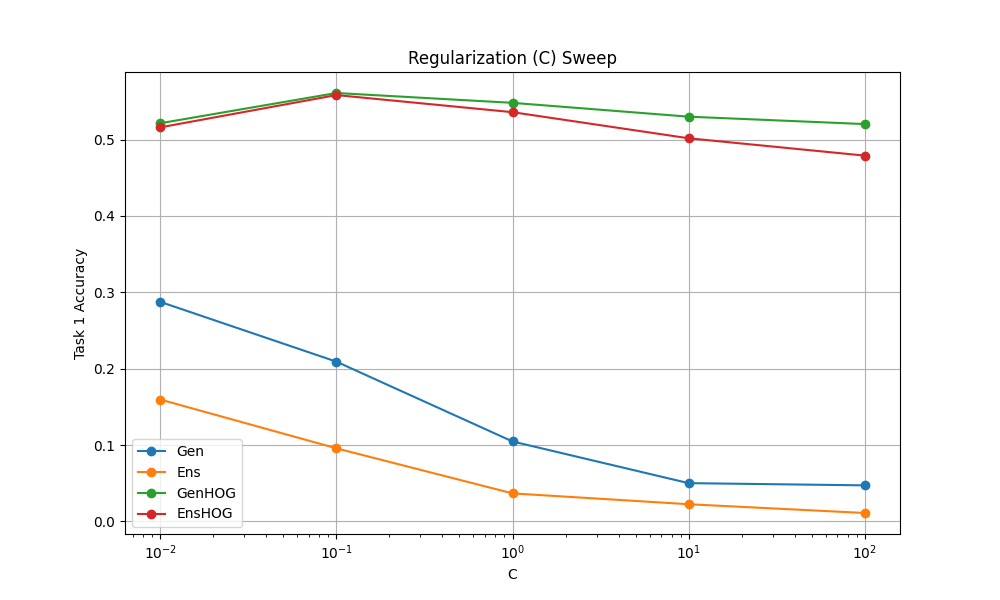
\includegraphics[width=0.5\textwidth]{images/image1.png}
\caption{\textbf{Sweep through different $C$ values to allow for a harder/softer margin.} Both the general HOG model and the ensemble HOG model perform best with $C = 0.1$, and both the general pixels model and the ensemble pixels model perform best with $C = 0.01$.}
\end{figure}

\begin{figure}[H]
\centering
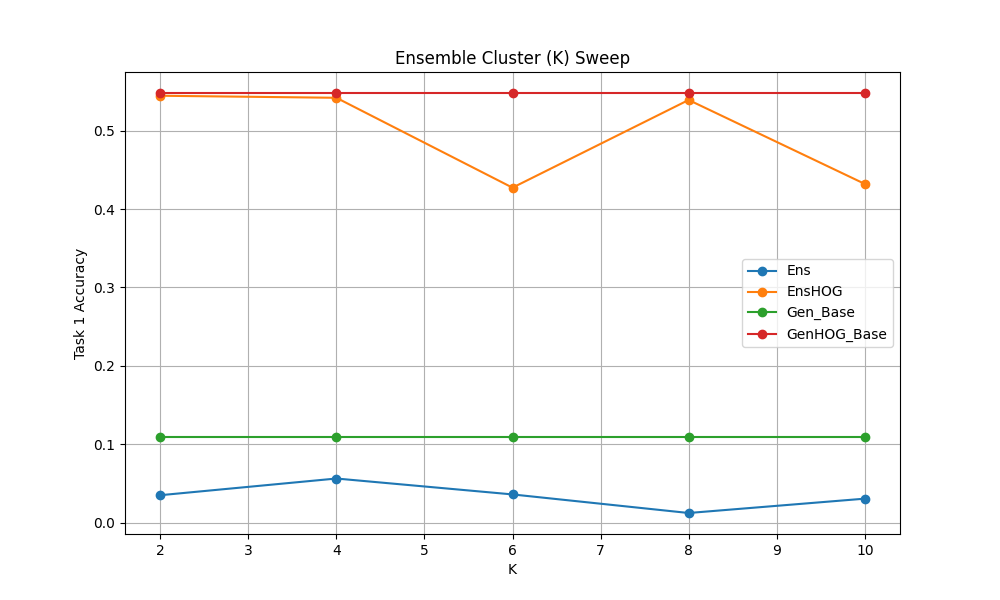
\includegraphics[width=0.5\textwidth]{images/image2.png}
\caption{\textbf{Sweep through different cluster numbers for the ensemble models.} The HOG ensemble performs best with two clusters, and the pixels ensemble performs best with four clusters. Note that with one cluster, performance would be identical between the general and ensemble models.}
\end{figure}

\begin{figure}[H]
\centering
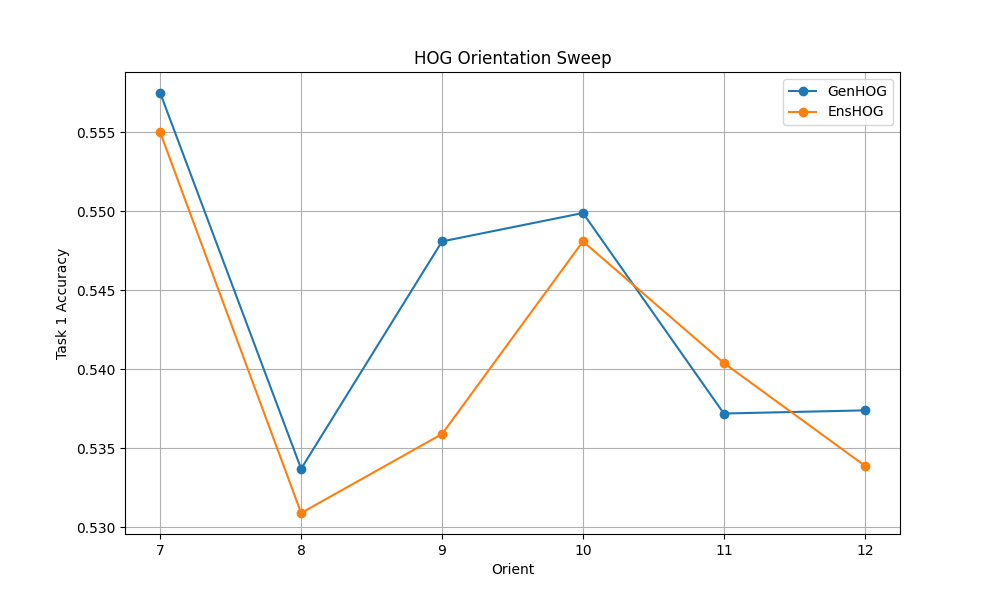
\includegraphics[width=0.5\textwidth]{images/image3.png}
\caption{\textbf{Sweep through different orientation numbers for the HOG models.} Both models perform best at classifying the character/symbol label for seven orientations.}
\end{figure}

\begin{figure}[H]
\centering
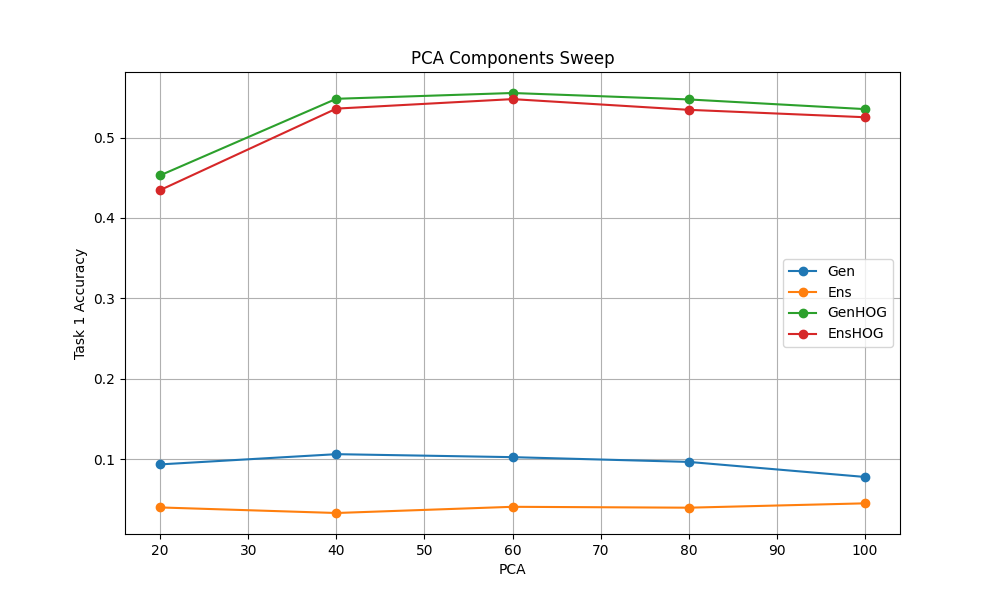
\includegraphics[width=0.5\textwidth]{images/image4.png}
\caption{\textbf{Sweep through different component numbers for PCA.} The two HOG models perform best with sixty components. The general pixel model performs best with forty components, and the ensemble pixel model performs best with 100 components.}
\end{figure}

\begin{figure}[H]
\centering
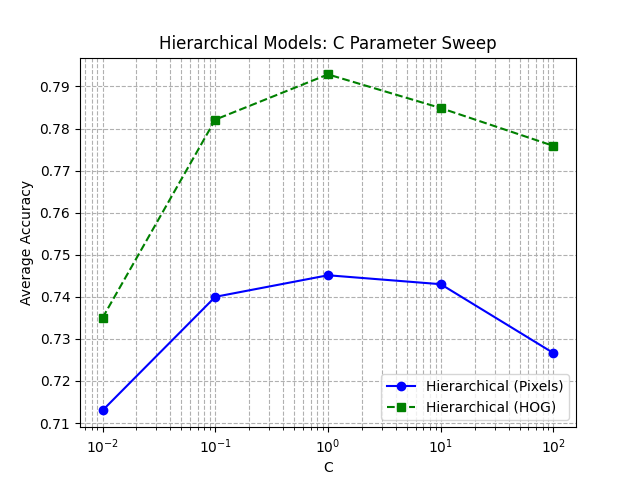
\includegraphics[width=0.5\textwidth]{images/image5.png}
\caption{\textbf{Sweep through different $C$ values for the hierarchical architecture.} Both of the models perform best with $C = 1$.}
\end{figure}

\begin{figure}[H]
\centering
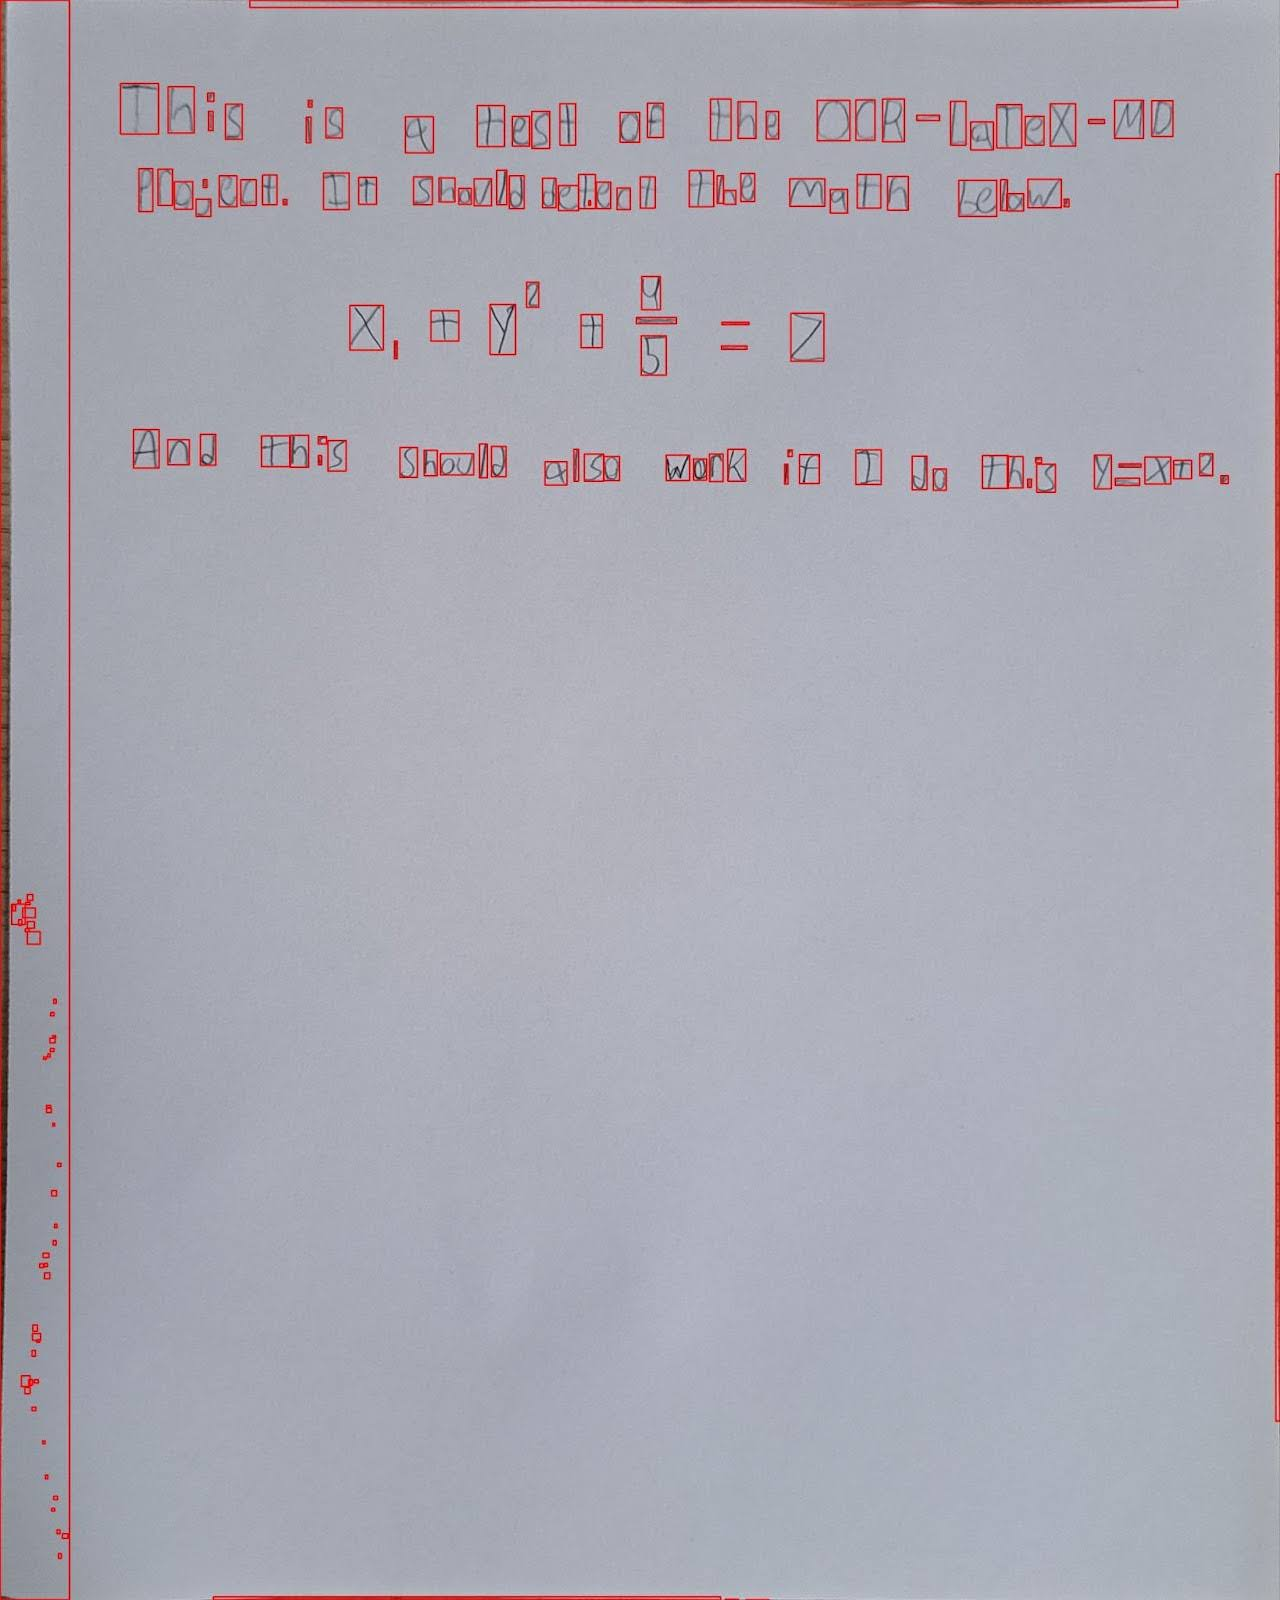
\includegraphics[width=0.5\textwidth]{images/image6.jpg}
\caption{\textbf{Example of the character segmentation algorithm.} There are some errors, notably when characters like ``i'' or ``='' are segmented into different letters.}
\end{figure}

\begin{figure}[H]
\centering
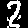
\includegraphics[width=0.5\textwidth]{images/image7.png}
\caption{\textbf{Example of a segmented character after processing.} It is clear to us what the character is, but there is also notable noise. Noise can throw off the SVM prediction because it messes with the HOG counts.}
\end{figure}

\begin{table}[H]
	\centering
	\begin{tabular}{|c|c|c|}
		\hline
		\textbf{Model}              & \textbf{Exact Match (\%)} & \textbf{CER (\%)} \\
		\hline
		\verb|Gen. SVM|          & 0                         & 141.38            \\\hline
		\verb|Ens. SVM|         & 0                         & 170.46            \\\hline
		\verb|Gen. HOG SVM|      & 0                         & 204.75            \\\hline
		\verb|HOG Ens. SVM|     & 0                         & 208.95            \\\hline
		\verb|Hier. SVM|     & 0                         & 159.28            \\\hline
		\verb|Hier. HOG SVM| & 0                         & 175.83            \\\hline
	\end{tabular}

	\caption{\textbf{Results table on MathWritingHandwritten and IAM-line for the SVM models.} Note that the CER is more than 100\% because of insertions and deletions. No models matched any of the samples correctly.}
\end{table}

\begin{table}[H]
	\centering
	\begin{tabular}{|c|c|c|}
		\hline
		\textbf{Model}         & \textbf{Exact Match (\%)} & \textbf{CER (\%)} \\
		\hline
		\verb|CNN-RNN|         & 32.28                         & 13.96                 \\\hline
		\verb|CNN-2RNN|        & 42.11                         & 12.25                 \\\hline
		\verb|CNN-Trans.| & 42.52                         & 18.88                 \\\hline
	\end{tabular}

	\caption{\textbf{Results table on MathWritingHandwritten and IAM-line for the neural network models.} The CNN-Transformer model performed best for exact match percent but was the worst for CER.}
\end{table}

\begin{figure}[H]
\centering
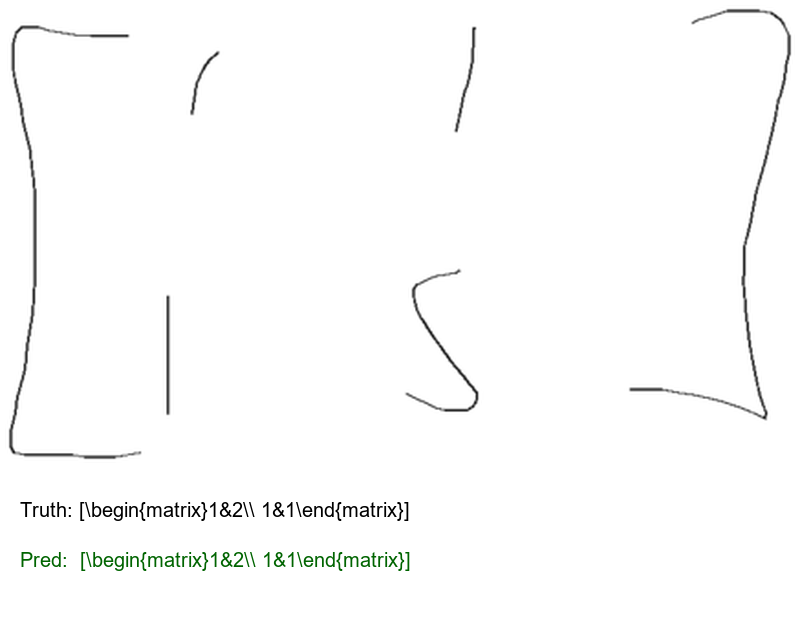
\includegraphics[width=0.5\textwidth]{images/image8.png}
\caption{\textbf{Sample correctly predicted matrix from the validation set by CNN-2RNN.} Note the handwritten line width. Also note the lack of spaces unless absolutely necessary.}
\end{figure}

\begin{figure}[H]
\centering
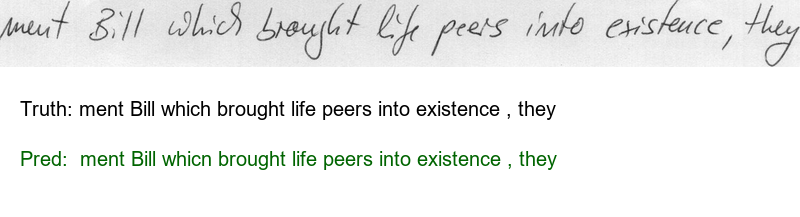
\includegraphics[width=0.5\textwidth]{images/image9.png}
\caption{\textbf{Sample correctly predicted text from the validation set by CNN-2RNN.} Note the handwritten line width. Also note the structural spaces put before punctuation.}
\end{figure}

\begin{figure}[H]
\centering
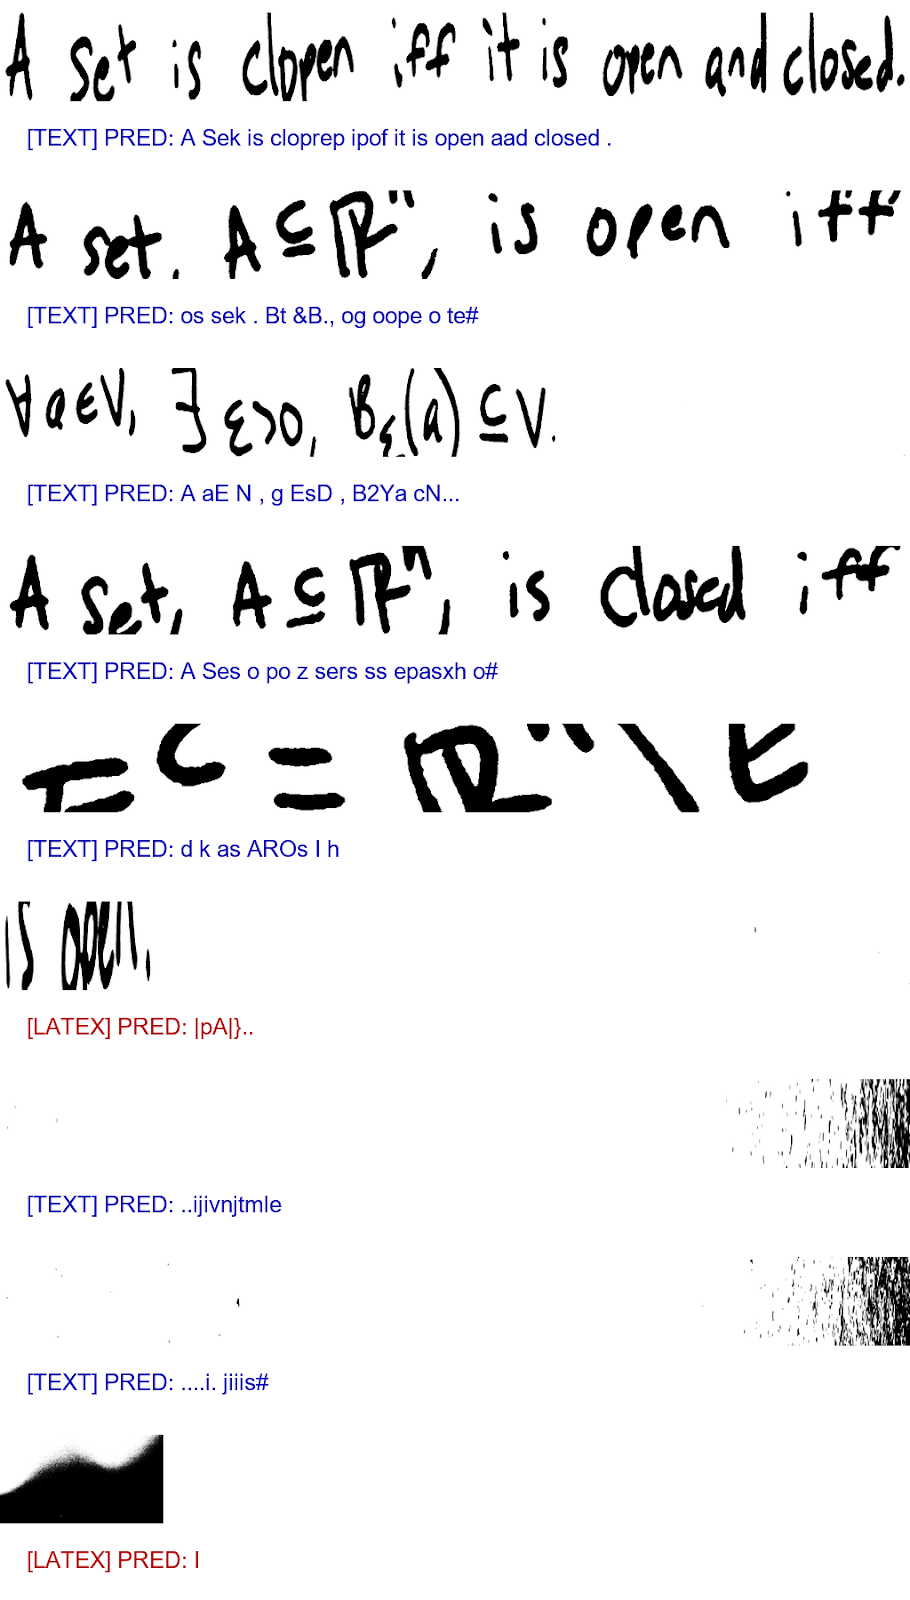
\includegraphics[width=0.5\textwidth]{images/image10.png}
\caption{\textbf{Full markdown text we segmented incorrectly predicted by CNN-2RNN.} Note the handwritten line width. Also note the struggles the segmentation algorithm has in noise, splitting LaTeX and text within the same line, and text sizing.}
\end{figure}

\section{Evaluation}

For SVM, there are two parts of the results to consider: training on characters/symbols and the full markdown performance. For the training results, the hierarchical model using HOG by far performed the best. This makes sense, given that HOG has been shown to help image classification and that it can greatly reduce the number of classes the model needs to have a decision boundary for, without coming with the higher risk of misfitting the true dataset.

Looking at the results of the ensemble SVM models, we believe that misfitting the data is a concern. In all tests we ran, the ensemble performed worse in both training and test accuracies than the respective general model. We believe this to most likely be caused by the lack of labels given to $k$-means. That is, if one category is split between two different clusters, the margin width maximization of SVM makes the decision boundary move, possibly in a way that worsens performance. We are disappointed that this did not work out, but given how many classes there are which are not dissimilar from each other (e.g., ``0'', ``O'', ``o'', and ``$\emptyset$'' are all very similar and could end up messing with clusters), it makes sense that this did not work as well as it does in other domains.

For the true task testing, we see significantly worse results, though this again makes sense. Given the noise problems all attempts at our segmentation algorithm had, we would anticipate bad results. That is, if our model is only predicting accurately ~80\% of the time in ideal scenarios (i.e., hierarchical HOG SVM with $C = 1$), we would expect, at best, a CER of 20\%, and then whatever problems are created as a result of the segmentation will only make this worse. Furthermore, CER is computed on the entire string, so unlike our accuracy on the training datasets where we are just computing if the character/symbol is correct or not, an incorrectly predicted LaTeX symbol inserts far too many characters (e.g., ``0'' is a single character, but ``\textbackslash emptyset'' is nine characters). This would explain why we have extra or too few characters predicted for an entire string. As a final note for the SVM model, even if the characters are independent of others' errors, a string of twenty characters and symbols to predict would be expected to work less than 1\% of the time ($0.8^{20}$) in the best case.

For the encoder-decoder architectures, we had better, but still not great results. The transformer did perform the best on the validation sets for exact match, but it also performed the worse in terms of CER. This could be because of the difficulty of spaces, where there was less loss for the transformer to just always follow the ``minimal spaces'' paradigm of LaTeX and be wrong with the text, especially when the text dataset added in so many extra spaces, such as before all punctuation.

The single decoder model performed the worst in terms of exact match accuracy, but still fairly okay in terms of CER. More than anything, this model serves as a point of reference for how the two decoder model performs.

The encoder-decoder model with two decoders performed really close to the transformer in terms of exact match but had significantly better CER. It also performed better in both exact match and CER than the single encoder model. This shows that, even with the added inaccuracies that a CNN router adds, having two separate decoders that each specialize in just one of the two datasets is a much better choice than a single decoder to do it all. As a result of the better CER performance, we used this model for testing on our own handwriting.

We believe that the neural models are not very generalized. Looking at the three different samples, we see why this struggles so much with generalization. The text in the MathWritingHandwritten dataset has very thin lines. The text in the IAM-line dataset is slightly thicker but still not as thick as our own handwriting was. The problem this causes is that the model struggles with the thicker characters and symbols that it does not have training data for.

This is not to say that it is completely bad. ``A Sek is cloprep ipof it is open aad closed.'' is not, in practice, that far off from ``A set is clopen iff it is open and closed.'' That said, we would need a more universal way to process our own handwriting to make the lines significantly thinner if we want to deploy this for our own use. You can also see the other segmentation problems that we have. While this was not a common occurrence, parts of text sometimes got clipped when segmenting the lines (this seemed particularly common when the handwriting was slightly rotated). There was also a large amount of noise picked up, particularly among the vignetting that naturally occurs at the corners of a picture.

\section{Future Work}

Going forward with the experience we have gained having conducted this experiment, there are a few paths we could go down to further expand on our concept. One path we could explore going forward is finding an alternative to the SVM method, which caused issues during the experimentation process. Specifically for SVM, the segmentation produced separate bounding boxes for singular expressions that are composed of separate lines, such as equal signs, where each line gets its own bounding box instead of one box that encapsulates the entire symbol. We could train a model, possibly a very lightweight CNN, that recognizes when individual figures comprise the same symbol, which would simplify the process greatly. This would be much more efficient for inference compared to the encoder-decoder architectures we used, especially with beam search instead of greedy decoding.

For the NN approach, the experiment would have greatly benefited from having more training time/more computing power, which would have likely increased its performance. Another avenue we could take moving forward would be to create separate models, instead of using separate decoders on a singular model. This would allow us greater flexibility in producing an output that more closely matches the text used to train our models, resulting in better performance and more accurate outputs. It would just require more training cost overall.

One approach we have seen used in other attempts at a similar project used a Generate-Compile-Fix loop, where after each produced pdf, any syntax issues are identified and remedied until a completely valid output is generated. Implementing this into our project would ensure that the final result is always valid from a syntax perspective, although there is no guarantee the generated syntax would match the expected output, only that it would have a valid structure. That is, the model would be forced to create an output that is actually usable in LaTeX, increasing the accuracy by preventing labels that we know are wrong because they do not compile.

One method we did not have time or money to test was how our model performs against larger pre-existing transformer-based models. It is possible that, given the size of these models, they would perform well on a task like this, although their performance would likely degrade with multi-page inputs as their context window dwindles, which is an advantage our model would have against them. Nevertheless, experimenting with these models may give us an insight into other avenues we could explore with our implementation by researching how they handle similar OCR tasks.

\section{Conclusion}

Having tried multiple approaches for this problem, there are some important takeaways that we can take going forward. Primarily, our mistake in using SVM for a sequence-based task. We spent too much critical time on this inefficient approach, when we now know that a neural encoder-decoder model drastically outperforms classical approaches (42\% Exact Match (EM) vs. 0\%).

Another roadblock in our implementation was that segmentation quality is a critical upstream dependency, as even a slight miscropping can drastically affect the final output. Noise is common in hand-written notes, especially when you are taking a picture of the notes, and we would need to take more precautions in handling this noise so the final output is not tainted by stray lines that are unimportant for the model to process. From our experimentation, it seems like the most successful approach was the CNN-2RNN, which offered the best balance of EM and CER. The transformer approach trades CER for EM gains, and the CNN-RNN just performs worse than CNN-2RNN in both metrics. As such, if we continue working on this to create a deployable model in the future, we will work starting from the CNN-2RNN model.

% Custom bibliography entries only
\bibliography{custom}

\end{document}
